\section{Experiments}%
\label{sec:experiments}

blabla

For both the Toy Data and the musdb18 dataset we experiment with prior models on time-domain and spectral-domain input.

In the full model each prior is used to extract its source channel separatly. Through their training they explicitly contract the density for the positive, in-class examples. During separation the priors therefore encounter negative, out-of-distribution samples for the first time. To be useful for separation, it is important that the priors give a low likelihood to samples from the other classes of the dataset.

\begin{marginfigure}
    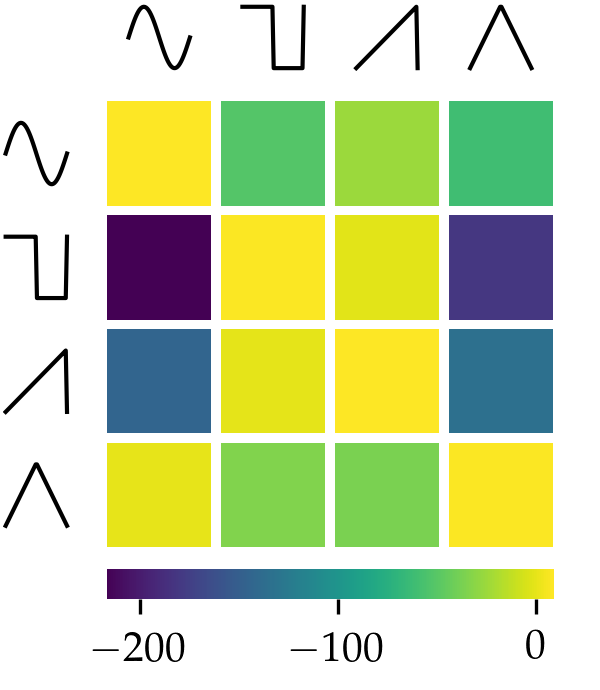
\includegraphics{heatmap_toy.png}%
    \caption{We display the mean average log likelihood of the test data under the different priors and the different signal sources.}%
    \label{fig:heatmap_toy}
\end{marginfigure}

We test for this by calculating the mean log likelihood of the the test data set under each prior, for each source channel separatly. What we anticipate is that the samples from the priors training source are of high likelihood while all other sources are low likelihood. In \cref{fig:heatmap_toy} we show the source dependent likelihoods for the Toy Data. The in-distribution samples are all of high likelihood while all out-of distribtion samples are highly un-likely. The Flow model therefore was able to detect out-of-distribution samples while only being trained on in-distribution samples~\footnote{Something psychological research has shown, humans being able to do.}. The estaimted densities are discriminative. When running the same experiment for the musdb18 the discriminative power is not hold up, see~\cref{fig:heatmap_musdb}. All signal sources are about equally likely under each prior density. We hypothesize this stems from the fact that the real musical data is severly more complicated compared to the Toy Data. The Flows model the appearance of sound in general, as the in-class variability of sounds is already high, without knowing anything about the \I{discriminative} differences between the instruments and does not infer the distribution from those features. Similar results were shown before in~\todo{cite some OOD VAE stuff}.

\begin{marginfigure}
    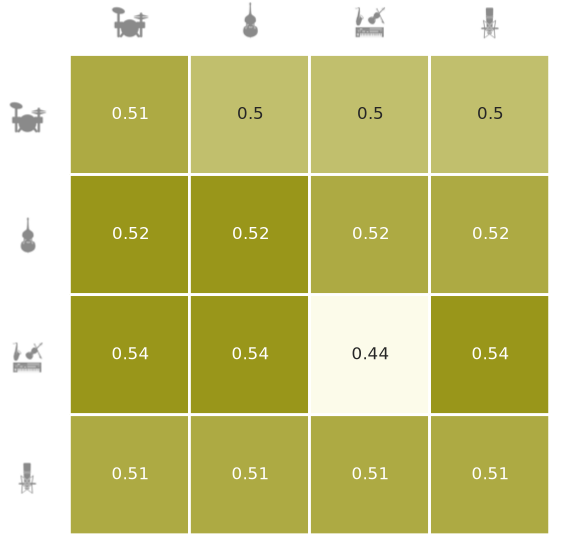
\includegraphics{heatmap_musdb.png}%
    % \caption{We display the mean average likelihood of the test data under the different priors and the different signal sources.}%
    \label{fig:heatmap_musdb}
\end{marginfigure}

The results for both datasets are similar for all tested model architectures and input domains. See Appendix~\todo{add results} for the full results.

With the prior models being not discriminative, it is not possible to train the separation model. Following we will try extend the priors to increase their discriminative power. Above that we propose that our method still holds merit given these results, further work on generative models might result in discriminative priors. The method can use any density as a drop-in replacement for the prior in the separation model.

As layed out in~\ref{Section methods} the bad out-of-distribution detection of generative models is not a suprising result and multiple recent works go about solving this. We want to increase the
